\documentclass[a4paper]{article}
\usepackage[utf8]{inputenc}
\usepackage[english]{babel}
\usepackage{amsmath} % per ambienti tipo cases
\usepackage{mathtools}
\usepackage{siunitx}
\usepackage{graphicx} % per includere figure
%\usepackage{subfigure}
\usepackage{booktabs} % per le tabelle
\usepackage{caption}
\usepackage{fancyhdr}
\usepackage{hyperref}
\usepackage[section]{placeins}
\usepackage{microtype}
\usepackage{caption}
\usepackage{subcaption}
\captionsetup[subfigure]{labelfont=rm}
\usepackage{verbatim} %multiline comments
\usepackage[backend=biber, style=numeric, safeinputenc, sorting=none]{biblatex}
\addbibresource{source.bib}	% uncomment for bibliography



%opening
\title{}
\author{}

\pagestyle{fancy}
\lhead{Musical Acoustics}
\chead{Homework 3}
\rhead{10743504, 10751919}
\newcommand{\Rarrow}{\mbox{\Large$\Rightarrow$}}

\begin{document}

\begin{titlepage}	
	\newcommand{\HRule}{\rule{\linewidth}{0.5mm}} % Defines a new command for horizontal lines, change thickness here
	
	\center % Centre everything on the page
	
	%------------------------------------------------
	%	Headings
	%------------------------------------------------
	
	
\includegraphics[width=.4\textwidth]{Logo_Politecnico_Milano.png}\\[0.4cm]
	\textsc{\LARGE}\\[0.3cm] % Main heading such as the name of your university/college
	
	\textsc{\large MSc. Music and Acoustic Engineering}\\[1cm] % Minor heading such as course title
	
	\textsc{\Large Musical Acoustics - A.Y. 2020/2021}\\[0.5cm] % Major heading such as course name
	
	%------------------------------------------------
	%	Title
	%------------------------------------------------
	
	\HRule\\[0.4cm]
	
	{\huge\bfseries Homework 3 - Sound Radiation from Plates}\\[0.4cm] % Title of your document
	
	\HRule\\[1.5cm]
	
	
	
	{\large\textit{Authors' IDs:}}\\
	10743504, 10751919, % Your name
	%\\ \textsc{Gruppo 11}
	
	%------------------------------------------------
	%	Date
	%------------------------------------------------
	
	\vfill\vfill\vfill % Position the date 3/4 down the remaining page
	
	{\large\today} % Date, change the \today to a set date if you want to be precise
	
	%------------------------------------------------
	%	Logo
	%------------------------------------------------
	
	\vfill\vfill
	%\includegraphics[width=0.2\textwidth]{Politecnico_di_Milano.eps}\\[1cm] % Include a department/university logo - this will require the graphicx package
	
	%----------------------------------------------------------------------------------------
	
	\vfill % Push the date up 1/4 of the remaining page
	
	
\end{titlepage}

\section{Adjusting the radiation cutoff by choosing the plate thickness}

Assuming an infinite plate, we can study the sound radiation by imposing that the air's velocity field and the plate velocity are equal on the plate's surface. This yields the following expression for the component of the acoustic wave vector normal to the surface:
$$ k_z = \omega \sqrt{\frac{1}{c^2} - \frac{1}{v_p^2}} $$
where $c$ is the sound velocity in air and $v_p$ is the velocity of the bending waves in the plate. Since bending waves in a plate are dispersive ($v_p \propto \omega^{\frac{1}{2}}$), the argument of the square root increases with frequency, which means there'll be a cutoff frequency below which $k_z$ becomes imaginary. In this case the solution for the acoustic field takes the form of a vanishing wave in the z direction, which doesn't carry any energy away from the plate's surface. Therefore, below the cutoff frequency there will not be any sound radiation.

In particular, the cutoff frequency is the one for which $v_p = c$. The velocity of the bending waves in a thin plate is:
$$ v_p(\omega) = \sqrt{\frac{\omega hc_L}{\sqrt{12}}} $$
where $c_L$ is the corresponding velocity of the quasi-longitudinal waves. For a wooden plate the longitudinal velocity depends on the direction of the wave; indicating with $x$ and $y$ the longitudinal and radial axes of the material respectively: 
\begin{align*}
	c_x = \sqrt{E_x /\rho(1 - \nu_{xy}\nu_{yx})} \qquad& c_y = \sqrt{E_y /\rho(1 - \nu_{yx}\nu_{xy})}
\end{align*}
where $\nu_{xy}$ and $\nu_{yx}$ are the Poisson's ratios relative to the two axes, while $E_x$ and $E_y$ are the Young's moduli.

The values of these parameters for Sitka spruce can be seen in Tab. \ref{tab:wood}, together with the resulting velocities. Since the longitudinal velocity is the highest of the two, waves that propagate in the $x$ direction will be cut off at a lower frequency than those that propagate in the $y$ direction. The cutoff frequency of the plate, therefore, is the one at which the velocity of the bending waves in the $x$ direction matches the speed of sound in the air. We can tune this frequency by varying the plate's thickness $h$: if we want a cutoff at $\SI{1.2}{\kilo\hertz}$, we will need to use a plate of thickness $h = \SI{9.5}{\milli\meter}$.

\begin{table}[h]
	\centering
	$\begin{array}{lllll|rr}
		\toprule
		E_x~[\si{\giga\pascal]}& E_y~[\si{\giga\pascal}] & \nu_{xy} & \nu_{yx} & \rho~[\si{\kilogram\per\meter\cubed}] & c_x~[\si{\meter\per\second}] &  c_y~[\si{\meter\per\second}]\\
		%\hline
		\midrule
		14.26 & 1.112 & 0.372 & 0.040 & 440 & 5.73\times10^3 & 1.60\times10^3\\
		\bottomrule
	\end{array}$
	\caption{Mechanical parameters of Sitka spruce, from \cite{wood}.}
	\label{tab:wood}
\end{table}

\section{Frequency dependence of the directivity}

The wave vector of the radiated wave lies on the $xz$ plane. The angle it forms with the plate's surface can be recovered by writing:
$$ \tan \theta = \frac{k_z}{k_x} = \sqrt{\frac{v_p^2}{c^2} - 1} $$

Much like before, the presence of $v_p$ in this expression implies a dependence on frequency of the direction of propagation. In Fig. \ref{fig:dir} we report a plot of the angle $\theta$ as a function of the frequency $f$.

\begin{figure}[h]
	\centering
	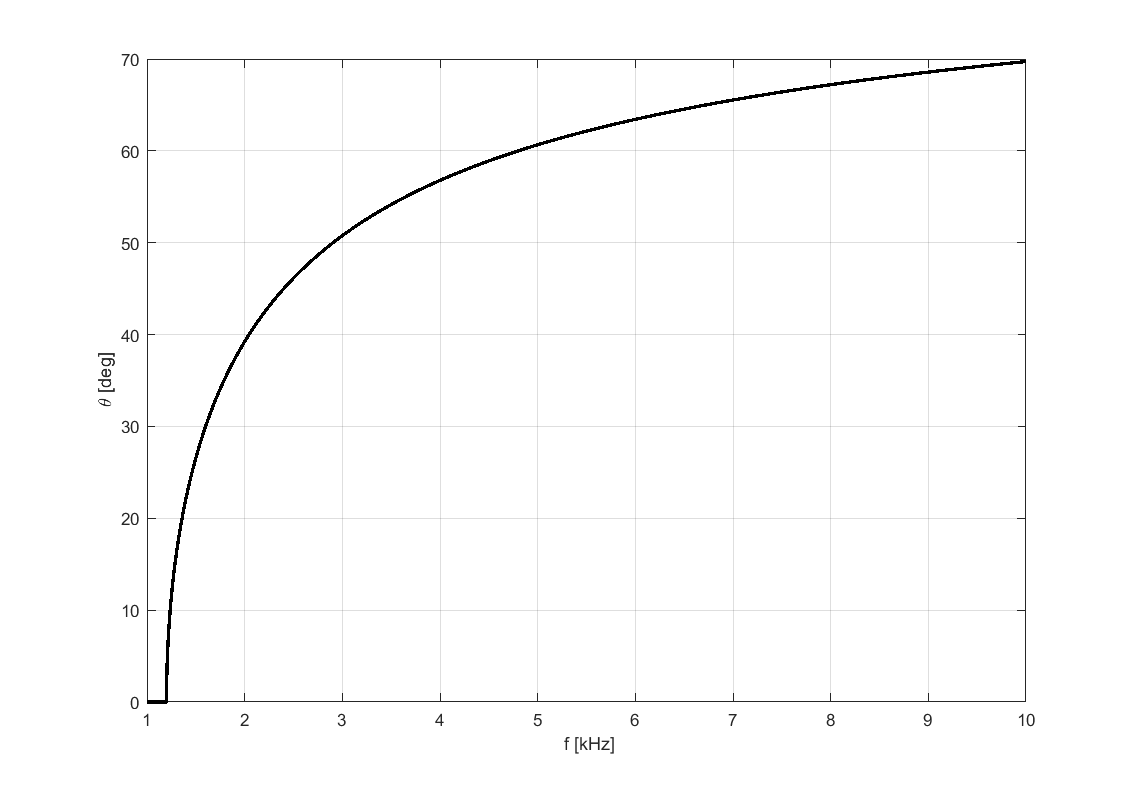
\includegraphics[width=0.8\linewidth]{lindir.png}
	\caption{Plot of $\theta$ as a function of $f$.}
	\label{fig:dir}
\end{figure}
Notice that what we are plotting here is actually the real part of the ratio $\frac{k_z}{k_x}$: this is why the graph is zero below the cutoff frequency.

\section{Effects of the finite extension of real plates}

Of course all the discussion presented up until now stands on the assumption that the plate we are considering is infinite in its extension. This is clearly a limiting case, but it can at least give us a picture of the expected radiating behavior of a real "large" plate, i. e. one in which the linear dimensions are all significantly greater than the wavelengths of interest. In a real plate, typically, the radiation spectrum will exhibit a roll-off below the theoretical cut-off frequency, as opposed to the discontinuity we have in the case of the infinite plate.

We can better understand what is happening by picturing the plate in a single mode as composed by different oscillating regions: for the infinite case, every one of these regions is surrounded by others moving with opposite phase, which cancel eachother's contribution to the radiation field. When the plate is finite, the presence of a boundary reduces this effect, particularly for lower modes, for which the wavelengths are comparable with the linear dimensions of the plate.

\printbibliography

\end{document}